\documentclass[output=paper]{langscibook}
\ChapterDOI{10.5281/zenodo.22796679}
\author{Markéta Malá\orcid{}\affiliation{Charles University}}
\title[\emph{Schodiště z mramoru} and \emph{the marble staircase}]{\emph{Schodiště z mramoru} and \emph{the marble staircase}: English divergent counterparts of Czech postmodifying prepositional phrases}
\abstract{The chapter explores the English translation correspondences of Czech postmodifying prepositional phrases, focussing on the rare cases of formal divergence. The contrastive analysis relies on material drawn from the parallel corpus InterCorp. The results reveal the impact of the register (fiction vs. non-fiction) and direction of translation on the degree of congruence between the counterparts. Drawing on both Czech texts translated into English (CS(en)) and English-to-Czech translations (cs(EN)), the study catalogues the recurrent patterns of correspondence and describes their formal and semantic properties. The choice of a particular divergent counterpart was found to be related mostly to the typological differences between Czech and English, as manifested, for instance, in the correspondence between Czech postmodifying prepositional phrases and English premodifying nouns or postmodification by participial clauses with semantically weak predicates.
\keywords{divergent translation counterparts, prepositional phrase, postmodification, parallel corpus, Czech, English}
}
\IfFileExists{../localcommands.tex}{
  \addbibresource{../localbibliography.bib}
  \usepackage{tabularx,multicol}
\usepackage{url}
\urlstyle{same}

 
\usepackage{langsci-optional}
\usepackage{langsci-lgr}
\usepackage{langsci-gb4e}

\usepackage{paralist}
\usepackage{enumitem}
\usepackage{cprotect}
\usepackage{fancyvrb}

\let\clipbox\relax
\usepackage[export]{adjustbox}
\usepackage{array}
\usepackage[normalem]{ulem}
\usepackage{langsci-branding}
\usepackage{langsci-bidi}
\usepackage[linguistics]{forest}

  
\makeatletter
\let\thetitle\@title
\let\theauthor\@author
\makeatother

\newcommand{\togglepaper}[1][0]{
   \bibliography{../localbibliography}
   \papernote{\scriptsize\normalfont
     \theauthor.
     \titleTemp.
     To appear in:
     E. Di Tor \& Herr Rausgeberin (ed.).
     Booktitle in localcommands.tex.
     Berlin: Language Science Press. [preliminary page numbering]
   }
   \pagenumbering{roman}
   \setcounter{chapter}{#1}
   \addtocounter{chapter}{-1}
}

\newbool{bookcompile}
\booltrue{bookcompile}
\newcommand{\bookorchapter}[2]{\ifbool{bookcompile}{#1}{#2}}

\newcommand{\qual}[1]{`#1'}
\newcommand{\bv}[1]{(\ref{#1})}

\newcommand{\ip}{ImPost}
\newcommand{\ipadv}{ImPost-adverbial}
\newcommand{\pradv}{ProxPost-adverbial}
\newcommand{\chisq}{Chi-squared}


% for rotated columns
\newcolumntype{T}[2]{%
    >{\adjustbox{angle=#1,lap=\width-(#2)}\bgroup}%
    l%
    <{\egroup}%
}
\newcommand*\rot{\multicolumn{1}{T{45}{1em}}}%


\VerbatimFootnotes


% \newcommand{\keywords}[1]{\textbf{#1}}


%  \newcommand{\textarabic}[1]{\RL{\arabicfont #1}}

  %% hyphenation points for line breaks
%% Normally, automatic hyphenation in LaTeX is very good
%% If a word is mis-hyphenated, add it to this file
%%
%% add information to TeX file before \begin{document} with:
%% %% hyphenation points for line breaks
%% Normally, automatic hyphenation in LaTeX is very good
%% If a word is mis-hyphenated, add it to this file
%%
%% add information to TeX file before \begin{document} with:
%% %% hyphenation points for line breaks
%% Normally, automatic hyphenation in LaTeX is very good
%% If a word is mis-hyphenated, add it to this file
%%
%% add information to TeX file before \begin{document} with:
%% \include{localhyphenation}
\hyphenation{
    par-a-digm
}

\hyphenation{
    par-a-digm
}

\hyphenation{
    par-a-digm
}

  \togglepaper[1]%%chapternumber
}{}

\begin{document}
\maketitle
%\shorttitlerunninghead{}%%use this for an abridged title in the page headers

\section{Postmodifying prepositional phrases}

\subsection{Introduction}

This study\footnote{This research was supported by the programme ‘Cooperatio – Linguistics’ (2022–26) implemented at Charles University.} examines the extent and types of correspondence between Czech postmodifying prepositional phrases (henceforth PPs) and their English translation counterparts. \citegen{Dušková2015} research into syntactic constancy of clause elements has shown that not only is the syntactic function of a modifier preserved in about 90\% of noun phrases translated from Czech to English, but also the form of the modification remains largely constant.\footnote{In the opposite, English > Czech direction, the ratio of noun modifiers translated by other clause elements was higher in \citegen{Dušková2015} sample, mainly due to factors connected with the head of the noun phrase and different forms of predication. The study did not focus on the degree of correspondence at the level of formal realization of the clause element.} Given the fact that in English PPs are “by far the most common type of postmodification” (\citealt{BiberEtAl2021}: 601), the choice of a non-prepositional English translation counterpart of a Czech postmodifying PP, such as \textit{postava v černé kombinéze} [\textit{…}] \textit{s dlouhým úzkým mečem v ruce} (‘\textit{figure} in black suit [\textit{…}] with long narrow sword in hand’) corresponding to \textit{a black-suited figure} [\textit{…}] \textit{holding a long narrow sword} in \REF{ex:mala:1}, may appear quite surprising. The present study sets out to explore the factors leading to such unusual correspondences.

\ea\label{ex:mala:1} CS. Z vody vystoupila postava \textit{v černé kombinéze} [figure in black overalls], s kyslíkovou bombou na zádech a \textit{s dlouhým úzkým mečem v ruce} [with a long narrow sword in hand]. (Michal Ajvaz, Druhé město, fiction)\footnote{The most relevant parts of the examples are highlighted in italics. All the examples were excerpted from the parallel translation corpus InterCorp (see Sources and \sectref{sec:mala:2}).}\\
en. Out of the water stepped \textit{a black-suited} figure with an oxygen cylinder on its back and \textit{holding a long narrow sword}. (transl. by Gerald Turner)
\z

\subsection{Prepositions and prepositional phrases}\label{sec:mala:1.1}

Prepositions and PPs are often relegated to the periphery of the grammatical description of a language, and denied “any real intrinsic syntactic interest other than as an annoying little surface peculiarity”. \citep[345]{Jackendoff1973} Nor do they appear to be a topic worth exploring from the lexical point of view – together with other synsemantic words they just “waste space in a dictionary”. \citep[81]{Sinclair1991} They have, however, received increasing attention since the 1990s with “the emergence of the field of lexico-grammar […], which recognizes the existence of a continuum between lexicon and grammar” (\citealt{CosmeGilquin2008}: 260), and corpus-driven phraseological research. Due to their high frequency, little formal variability, and wide distribution across various registers, prepositions can serve as a useful starting point to “reveal phraseologies that are linked to recurrent meanings and functions rather than to subject-matter”. \citep[292]{Hunston2008} Prepositions have been found to constitute parts of multi-word lexico-grammatical sequences, or patterns, which can, for instance, distinguish among registers (e.g., \citealt{ScottTribble2006}; \citealt{Hunston2008}; \citealt{Groom2010}), or reveal disciplinary variation in academic writing \citep{Groom2010}.

Prepositions are a synsemantic word class. In both Czech and English, they are most typically complemented by nouns or noun phrases (\textit{in a street}, \textit{na ulici}). Other types of complements include adverbs (\textit{from abroad}, \textit{na potom} ‘for afterwards’), and in English also nominal clauses, finite and non-finite (\textit{instructions on where they are used}, \textit{three days after leaving Darwin}), or other PPs (\textit{from behind the wire fencing}). In Czech, the preposition determines the case of its complement. In English, this applies only to pronouns; “those pronouns that have different (non-genitive) case forms almost invariably appear in the accusative after prepositions” (\citealt{HuddlestonPullum2002}: 598). While in Czech the preposition always precedes its complement, in English, the preposition can be ‘stranded’, i.e. not followed by its complement, in such constructions as interrogative or relative clauses (e.g., \textit{What more could a child ask for?}) (\citealt{BiberEtAl2021}: 108–110, \citealt{CvrčekEtAl2010}: 333), and “occasionally, a preposition is postposed, as in the case of English \textit{ago} (e.g., \textit{three weeks ago})” \citep[147]{Hasselgård2021}.

From the syntactic point of view, prepositions perform three basic functions, as illustrated in \REF{ex:mala:2}. They express the relation

\begin{itemize}
\item between the verb or adjective and a nominal expression, where the nominal element typically constitutes a valency complement of the verb (the object) or the adjective, e.g., the relation between \textit{wondered} and the noun phrase \textit{the acuteness of the symptoms};
\item between two nominal expressions, e.g., between the noun phrases \textit{the acuteness} and \textit{the symptoms}; or
\item between the adverbial and the proposition conveyed by the clause, e.g., between the adverbial \textit{at the time} and the rest of the clause (cf. \citealt{Čermák1996}: 32, \citealt{BiberEtAl2021}: 109).
\end{itemize}

\ea\label{ex:mala:2}
EN. \textit{At the time}, I […] merely wondered \textit{at the acuteness of the symptoms} (Robert Louis Stevenson, The Strange Case of Dr Jekyll and Mr Hyde, fiction)
\z

\citet[76]{BiberEtAl2021} use the term ‘bound prepositions’\footnote{More precisely, the terms ‘bound’ and ‘free’ prepositions refer to uses of prepositions, since some prepositions can be used either as ‘bound’ valency complements or as ‘free’ prepositions (cf. one had to rely \textit{on} intuition \textit{–} we were sitting \textit{on} the terrace).} to refer to the prepositions which “have little independent meaning, and the choice of the preposition depends upon some other word (often the preceding verb)”\footnote{The close relationship between the verb and the preposition is also reflected in the fact that the ‘verb + preposition’ combinations “such as \textit{confide in}, \textit{rely on}, and \textit{part with} are usually regarded as forming a multi-word unit and are called prepositional verbs” (\citealt{BiberEtAl2021}: 76)}.  (i.e. type a, and partly b above). ‘Free prepositions’ on the other hand, “have an independent meaning; the choice of the preposition is not dependent upon any specific words in the context” (type c above). Bound prepositions, therefore, enter a bidirectional relationship – their choice is dependent on the valency of the verb, adjective or noun, and at the same time, they determine the choice and form of their own complement \citep[33]{Čermák1996}.

The present chapter focuses on the adnominal uses of prepositions, namely PPs which postmodify a noun.  In Czech grammar, the modifier in the noun phrase is termed ‘přívlastek’ or ‘atribut’ (‘attribute’), an optional element modifying a syntactic noun (\citealt{Dušková1999}: 209, cf. \citealt{ŠtíchaEtAl2013}: 725). PPs are a form of the ‘non-congruent attribute’, i.e. a postmodifier which does not display grammatical agreement with the head noun (\citealt{GreplEtAl1995}: 503). The choice of the preposition can be dependent on the valency of the head noun, e.g., \textit{přednáška o syntaxi} ‘a lecture on syntax’. Free postmodifying PPs express various circumstances, characterizing the head noun, such as the place (\textit{slavnost na zahradě} ‘a party in the garden’), time (\textit{noci v létě} ‘nights in summer’), or origin (\textit{svetr z vlny} ‘sweater from wool’). \citet[509]{GreplEtAl1995} point out that the postmodifying phrase often corresponds to adjectival premodification (e.g., \textit{zahradní slavnost} ‘garden party’, \textit{letní noci} ‘summer nights’, \textit{vlněný svetr} ‘woolen sweater’). However, the relationship between the noun and the modifier is expressed more explicitly by the preposition, cf. \textit{kuchyňský nůž} (‘a kitchen knife’) and \textit{nůž v kuchyni / z kuchyně / pro kuchyň} (‘a knife in/from/for the kitchen’) (\citealt{Čermák1996}: 33, cf. \citealt{ŠtíchaEtAl2013}: 730–734, \citealt{Karlík2017}).

In English, “[p]repositional phrases are by far the most common type of postmodification”, making up “65–80\% of all postmodifiers in all registers” (\citealt{BiberEtAl2021}: 601). As mentioned above, the choice of the preposition can be constrained by the preceding noun valency, e.g., \textit{her reliance on public support}.

\subsection{A cross-linguistic view of postmodifying prepositional phrases}

As shown by \citet[147]{Hasselgård2021}, “[c]ontrastive studies of the syntactic functions of prepositional phrases indicate that languages may have different restrictions and preferences regarding their use even when the linguistic resources are similar”. Considering the postmodifying PPs, the differences may involve, for instance, their overall frequency (\citealt{Dušková2015}, \citealt{Hasselgård2021}), their degree of flexibility \citep{Moreira-Rodrigues2006}, the restrictions on the use of a particular semantic group of postmodifiers \citep{Mott2013}, or the polysemy and phraseology of individual prepositions (\citealt{CosmeGilquin2008}, \citealt{Schmied1998}).

The degree of translational equivalence of PPs is likely to be influenced by the syntactic function of the PP (\citealt{CosmeGilquin2008}, \citealt{Schmied1998}). For example, Cosme \& Gilquin’s (2008: 270) results suggest that postmodifying \textit{with-}PPs tend to have congruent French counterparts (e.g., \textit{its strategic relationship with Syria} corresponding to \textit{sa relation stratégique avec la Syrie}) much more frequently than when they occur in other syntactic functions.\footnote{This may be connected with the fact that in postmodification, the preposition tends to express “the prototypical sense of mutual relation, rather than the more metaphorical senses which are characteristic of \textit{with}”. (\citealt{CosmeGilquin2008}: 271)} Therefore, when exploring the cross-linguistic correspondences of PPs, the comparison cannot be purely formal, but should “concern the mapping between form and function” \citep{Gast2012}. At the same time, “[the] degree of congruence in translation differs across translation directions” \citep[159]{Hasselgård2021}.

For the English translation counterparts of Czech PPs, “the general distribution of equivalents is typically in the proportion of 2:1 (two prepositional equivalents to one non-prepositional)” (\citealt{KlégrMalá2009}: 17). The range of prepositional equivalents is quite broad, usually with one dominant preposition both in terms of frequency\footnote{The frequency of the dominant counterpart appears to be different for each preposition. For instance, 49.7\% of instances of the Czech preposition \textit{v/ve} were translated using its dominant counterpart, the English preposition \textit{in}, and 18\% of \textit{po} by the dominant preposition \textit{after} in \citegen{KlégrMalá2009} data.} and the number of senses it can translate (e.g., \textit{in} for \textit{v/ve}). The degree of formal congruence of the translation counterparts appears to be related to the syntactic function of the PPs, with postmodifying and adverbial PPs being translated by congruent counterparts more frequently (65–70\% of counterparts) than those functioning as complements.

Postmodification, generally, “displays correspondence [between Czech and English] not only in the syntactic function but also in the form of realization” \citep[136]{Dušková2015}. Where postmodification is realized by a PP in Czech, the English translation was found to be congruent both syntactically and formally in a vast majority of correspondences (see \sectref{sec:mala:1.1}), with most divergent counterparts comprising premodification by a converted noun, e.g., \textit{přiznání k dani – tax return} (\citealt{Dušková2015}: 142–145). The correspondence between a Czech postmodification by a PP and an English premodification by a converted noun – “a formally indeterminate word class acquiring its syntactic function from its position” \citep[159]{Dušková2015} – reflects the typological distinctions between the two languages, and the analytic and nominal character of English in particular.

The premodifying nouns, as well as adjectives, were also listed by Klégr et al. \citealt[178–180]{klegr_anglicke_2012} as possible non-prepositional correspondences of postmodifying PPs comprising the prepositions \textit{v/ve} ‘in’, \textit{na} ‘at’ and \textit{s/se} ‘with’, e.g., \textit{tik ve tváři} {\textup{‘a} }{\textup{tic in face}}’ \textit{– facial tic}, \textit{dopis na rozloučenou} ‘a letter for farewell’ \textit{– a farewell letter}, \textit{pouzdro s pistolí} {\textup{‘a} }{\textup{holster with pistol}}’ \textit{– pistol holster}. The postmodifying \textit{v/ve}, \textit{na} and \textit{s/se} PPs were also found to be translated by participial postmodifiers, e.g., \textit{křeslo v kombinaci dřeva a kůže} ‘a chair in a combination of wood and leather’\textit{– chair made of wood and leather}, \textit{pohled na zelené dálky} ‘a view of green distances’ \textit{– a distant view clothed in fresh green}, \textit{košík s malým Mojžíšem} {\textup{‘the} }{\textup{basket with little Moses}}{\textit{’}} \textit{– the basket carrying little Moses}.

As the above studies have shown, the translation correspondences where a Czech postmodifying PP has a non-prepositional English counterpart are rare. This appears to be mainly due to two factors: first, the constancy of syntactic function and realization form of postmodification in translation from Czech to English \citep{Dušková2015}, and secondly, the typological differences between the predominantly synthetic Czech language and analytic English.  In Czech, the relation between two nouns within the noun phrase is conveyed most frequently by a case marking of the modifying noun (\citealt{ŠtíchaEtAl2013}: 728), cf. \textit{kousek čokolády} ‘piece-\textsc{nom} chocolate-\textsc{gen}’– \textit{a bar of chocolate}; \textit{procházka lesem} ‘walk-\textsc{nom} forest-\textsc{instr}’– \textit{a walk in the forest}). In the English noun phrase, on the other hand, the preferred means of expressing the relation between the head noun and the postmodifier is the preposition, PPs constituting the most frequent form of postmodification (\citealt{BiberEtAl2021}: 601). Alternatively, the modifying function of the noun can be indicated by word order in English, with the modifier preceding the head noun, e.g., \textit{čokoládové tyčinky} (‘chocolate-\textsc{adj} bars-\textsc{noun}’) – \textit{chocolate bars}, \textit{lesní cesta} (‘forest{}-\textsc{adj} path-\textsc{noun}’) – \textit{a forest path}. As the examples illustrate, in Czech the corresponding premodifier is expressed by a denominal adjective. In Czech, conversion is a marginal word-formation process, and premodifying nouns are limited to loanwords (e.g., \textit{jazz klub}, \textit{fit centrum}), abbreviations (e.g., \textit{IBM diskety}, \textit{HIV test}) and expressions bordering on apposition (e.g., \textit{chudák Marie} ‘poor{}-\textsc{noun} Mary-\textsc{noun}’) (\citealt{Veselovská2017}, \citealt{Karlík2017}). In English, using the noun as a premodifier requires no morphological changes in the noun. Due to the fixed word-order, including the ordering of the components of the phrase, the modifying function of the noun is sufficiently indicated by its position within the noun phrase. This may be further supported by the loss of the grammatical contrast of number, e.g., \textit{child labour}, \textit{trouser leg} (\citealt{DuškováEtAl2009}: 2.22.21).

\section{Material and method}\label{sec:mala:2}

The analysis presented in this chapter focuses on the English translation correspondences of Czech postmodifying PPs with the seven most frequent Czech prepositions – \textit{v} ‘in’, \textit{na} ‘at’, \textit{z} ‘from’, \textit{s} ‘with’, \textit{o} ‘about’, \textit{do} ‘to’, and \textit{k} ‘towards’ (\citealt{CvrčekEtAl2010}: 333). The queries\footnote{The basic form of the query was [tag="N.+"][lemma="v{\textbar}na{\textbar}z{\textbar}s{\textbar}o{\textbar}do{\textbar}k"]} also included the vocalized forms of the prepositions – \textit{ve}, \textit{ze}, \textit{se}, \textit{ke}, \textit{ku} – which are used when the following word starts with the same or similar consonant as the preposition, or with a consonantal cluster, e.g., \textit{ve vesmíru} ‘in space’, \textit{ke stromu} ‘towards the tree’ (\citealt{CvrčekEtAl2010}: 340–341).

The research was conducted in two steps, exploring:

\begin{enumerate}
  \item the impact of the direction of translation (CS > en, or EN > cs), and the register (fiction and non-fiction) on the choice of the English counterparts of Czech postmodifying PPs (Step 1), and
\item the types of divergent counterparts of a Czech postmodifying PP (Step 2).
\end{enumerate}

Methodologically, the research falls within corpus-based contrastive studies. The phenomenon under study is a rare one. The method adopted therefore aims primarily at identifying, describing and classifying the relevant patterns of translation correspondence, rather than at providing a comprehensive overview of their distribution and frequency.

\subsection{Step 1}

In order to explore the impact of both the register and the direction of translation, four subcorpora of the corpus InterCorp v14 were compiled: fiction translated from Czech to English and from English to Czech, and non-fiction in both directions of translation. The size of the subcorpora is given in \tabref{tab:mala:1}. All texts available in the respective categories in InterCorp v14 were used, which resulted in incomparable sizes of the fiction and non-fiction subcorpora. This, however, does not seem to pose a major problem for the present study due to the methods adopted (i.e. working with samples in Step 1, and using the corpus as a repository of examples extracted by individual queries in Step 2).

\begin{table}
\begin{tabularx}{\textwidth}{QlYYY}
\lsptoprule
{Direction of translation} & {Register} & \multicolumn{3}{c}{ {Size of the subcorpus}}\\
\cmidrule{3-5}
&  & {Number of positions} & {Number of texts} & {Number of authors}\\
\midrule
 CS(en) & fiction &  4,686,413 &  56 &  31\\
& non-fiction &  611,658 &  5 &  5\\
 cs(EN) & fiction &  25,258,196 &  215 &  138\\
%\hhline%%replace by cmidrule{-~~~~}
& non-fiction &  2,567,506 &  21 &  17\\
\lspbottomrule
\end{tabularx}
\caption{The size of the four subcorpora of InterCorp v14 (Step 1 of the research).}
\label{tab:mala:1}
\end{table}

The Czech texts (originals and translations) in the four subcorpora were searched for contiguous sequences of a noun and one of the prepositions \textit{v/ve} ‘in’, \textit{na} ‘at’, \textit{z/ze} ‘from’, \textit{s/se} ‘with’, \textit{o} ‘about’, \textit{do} ‘to’, and \textit{k/ke/ku} ‘towards’. The results were shuffled and checked manually\footnote{The cases of omission of the modifier resulting in a meaning shift and free translations, where the extent of divergence from the source at clausal level made it impossible to identify the counterpart of the postmodifying PP, were discarded.} in order to select only postmodifying PPs and discard the chance sequences of a noun and adverbial \REF{ex:mala:3}. Cases of comitative coordination (\citealt{Škrabalová2011}, cf. \citealt{CechovaEtAl_2011_CestinaRec}: 320), i.e. “a paratactic relationship between noun phrases syntactically framed as hypotaxis using the preposition \textit{s/se}” \citep[207]{Malá2017}, illustrated by \REF{ex:mala:4}, were also removed from the dataset.

\ea\label{ex:mala:3}
CS. Šarceceg vyhodila zbytky \textit{kozy z okna} […] (Petra Hůlová, Paměť mojí babičce, fiction)\\
en. Shartsetseg threw the \textit{goat out the window} […] (transl. by Alex Zucker)
\z

\ea\label{ex:mala:4}
CS. I \textit{Eva s Marií} [Eva with Marie] se usmívají. (Michal Viewegh, Vybíjená, fiction)\\
en. \textit{Eva and Marie} were also smiling. (transl. by David Short)\\
\z

In some cases, “it may be difficult to decide whether a prepositional phrase following a noun is a postmodifier of the noun or an adverbial in the clause”. (\citealt{BiberEtAl2021}: 109) In \REF{ex:mala:5}, the PP \textit{na koncích propletených ramen lustru} (‘at the ends of the interlacing branches of a chandelier’) could be analyzed as either an adverbial (specifying the location of ‘coming on’, cf. the English translation) or a postmodifier of the noun \textit{světla} (‘lights’) (specifying the location of the lights). Such concordance lines were retained, and analyzed as postmodifiers.

In noun phrases with multiple postmodification the difference in the relative position of the postmodifying PP was neglected as long as its correspondence to an English counterpart could be established.\footnote{Examples of multiple postmodification, e.g., EN. přezkoumat poslední \textit{reakce Douga-8612 na tuto zkušenost} [reactions by Doug-8612 to this experience] (Philip Zimbardo, The Lucifer Effect, fiction) – cs. \textit{review the final reactions to this experience by Doug-8612} (transl. by Radek Kašpar and Marika Králíková), reveal the close relationship between the Czech head noun and postmodifying genitive (\textit{Douga-8612}), which is reflected in its obligatory position immediately after the noun (cf. \citealt{DuškováEtAl2009}: 14.13.2).}

\ea\label{ex:mala:5} CS. Náhle se pode mnou rozsvítila světla \textit{na koncích propletených ramen lustru}, visícího na dlouhém laně, které bylo upevněné k lucerně kupole hned vedle mé hlavy; […] (Michal Ajvaz, Druhé město, fiction) \\
en. Suddenly lights came on \textit{at the ends of the interlacing branches of a chandelier} hanging from a long cable attached to the turret of the cupola right next to my head; […] (transl. by Gerald Turner)
\z

From the Czech texts in each subcorpus, relevant clauses comprising postmodifying PPs were excerpted together with their English translation counterparts until a sample of 250 clauses from each subcorpus was compiled. The representation of the individual prepositions in the 1,000-clause sample is given in \tabref{tab:mala:2}. The relative frequency and the types of counterparts will be discussed in \sectref{sec:mala:3}.

\begin{table}
\begin{tabularx}{\textwidth}{lYrYrY}
\lsptoprule
 {Preposition} & \multicolumn{2}{c}{ {Fiction}} & \multicolumn{2}{c}{ {Non-fiction}} & {Total}\\
 \cmidrule(lr){2-3}\cmidrule(lr){4-5}
& {CS(en)} & {cs(EN)} & {CS(en)} & {cs(EN)} & \\
\midrule
{v} ‘in’ &  54 &  62 &  68 &  64 &  248\\
{do} ‘to’ &  6 &  8 &  9 &  4 &  27\\
{k} ‘towards’ &  14 &  14 &  33 &  12 &  73\\
{na} ‘at’ &  54 &  59 &  50 &  51 &  214\\
{o} ‘about’ &  24 &  16 &  28 &  34 &  102\\
{s} ‘with’ &  56 &  38 &  23 &  45 &  162\\
{z} ‘from’ &  42 &  53 &  39 &  40 &  174\\
{Total} &  250 &  250 &  250 &  250 &  1,000\\
\lspbottomrule
\end{tabularx}

\caption{The representation of the 7 most frequent Czech prepositions in the sample of fiction and non-fiction text, Czech originals, and translations from English.}
\label{tab:mala:2}
\end{table}

\subsection{Step 2}

As the divergent counterparts of postmodifying PPs are quite rare in both directions of translation, it was obvious that more data was needed to explore and describe the types of non-prepositional counterparts in detail. A larger, more recent version 15 of the corpus InterCorp\footnote{Two subcorpora of InterCorp v15 were compiled and used, one comprising Czech original fiction and non-fiction texts and their English translations (5,612,530 tokens, CS(en)), the other English fiction and non-fiction source texts and their Czech translations (29,975,445 tokens, cs(EN)).} was used, and more specific queries based on the findings of Step 1 were formulated to identify further instances of the various types of counterparts (e.g., a sequence of a noun and one of the prepositions in question in the Czech text corresponding to a sentence comprising two adjacent nouns in English), relying on the corpus as an “example bank”. (\citealt{LüdelingKytö2008}) Since this step focussed on the qualitative description rather than on the frequency of the types of counterparts, the direction of translation and the register were disregarded. The results will be discussed in Section 4.

\section{The counterparts of Czech postmodifying prepositional phrases (Step 1)}\label{sec:mala:3}

\subsection{Congruent and divergent counterparts}\label{sec:mala:3.1}

The overall majority of counterparts of the Czech postmodifying PPs (76.6 \%, 766 instances) were formally congruent. The highest degree of divergence could be observed in Czech translations of English fiction; in non-fiction, generally, formally divergent counterparts were rarer than in fiction\footnote{In either direction of translation, the differences in the representation of non-prepositional counterparts between fiction and non-fiction are not statistically significant at the level of p < 0.05 (log-likelihood, calculated using llwizard available at https://ucrel.lancs.ac.uk/llwizard.html).} (\figref{fig:mala:1}), perhaps reflecting the higher degree of standardization of non-fiction texts (cf. \citealt{KufnerováEtAl1994}: 16).

\begin{figure}
 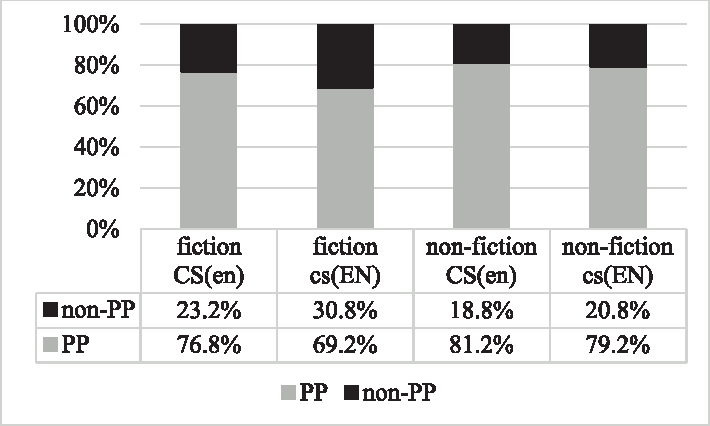
\includegraphics[width=\textwidth]{figures/4_Mala_figure 1mod.pdf}
\caption{\label{fig:mala:1} Formally congruent (PP) and divergent (non-PP) correspondences of Czech postmodifying PPs (samples of 250 occurrences for each sub-corpus)}
\end{figure}

Most of the formally congruent counterparts (92.2 \%; i.e. 706 out of the 766 instances) also performed the same, postmodifying syntactic function as the Czech PP \REF{ex:mala:6}. Again, the degree of syntactic divergence was highest between English original fiction texts and their Czech translations. In both text-types and directions of translation, most of the syntactically non-congruent counterparts (6.4\%, 49 instances) consisted in the Czech head noun corresponding to an English verb or predicative adjective. The English PP functioned as the adverbial or complement of the verb (often non-finite) or adjective \REF{ex:mala:7}. A minor type of syntactically divergent prepositional counterpart was represented by complex prepositions (1.4\%, 11 instances), e.g., \textit{v závislosti na pojetí jazyka} ‘in dependence on the conception of language’ \textit{– according to conceptions of language}.


\ea\label{ex:mala:6} CS. Jeho \textit{pohled na funkce} [view of the functions] jazyka […] založil nový směr ve filozofii jazyka a lingvistice vůbec. (František Čermák, Základy lingvistické metodologie, non-fiction)\\
en. His \textit{view of the function} of language […] established a new trend in the philosophy of language and linguistics generally […]. (transl. by Patrick Corness)
\z

\ea\label{ex:mala:7}
cs. Obstoupily ho kolem dokola a zahrnuly ho \textit{nářky na své bolesti} [complaints about their aches] a potíže a nejrůznější ženské neduhy. (transl. by Zuzana Mayerová)\\
EN. They clustered around him, \textit{complaining about their aches} and pains and their various female ills.  (Isaac Bashevis Singer, The Family Moskat, fiction)
\z

The following sections will focus merely on correspondences between Czech postmodifiers realized by PPs and their formally divergent English counterparts (both in non-translated and in translated texts), i.e. English counterparts whose realization form is not a PP, and which may perform a variety of syntactic functions.

\subsection{Classification of formally divergent translation correspondences of Czech postmodifying prepositional phrases}\label{sec:mala:3.2}

The non-prepositional translation correspondences of the Czech postmodifying PPs (both CS and cs) can be classified into three groups according to the syntactic function of the English counterpart:

\begin{itemize}
\item Premodifiers, e.g., CS. dárek k \textit{narozeninám} ‘a present for birthday’ \textit{–} en. a \textit{birthday} present;
\item non-prepositional postmodifiers, e.g., CS. jednání \textit{v Moskvě}  ‘talks in Moscow’ \textit{–} en. the talks \textit{held in Moscow};
\item complements of a verb which corresponds to the head noun of the Czech noun phrase, e.g., CS. v pohádce […] je \textit{zmínka o svatbě královského sourozeneckého páru} ‘a mention of a royal sibling-marriage’ – en. the tale […] \textit{mentions a royal sibling-marriage}).
\end{itemize}

Apart from these types, two further classes were distinguished which involve indirect translation techniques – reduction and merged counterparts.

\begin{itemize}
\item  Reduction consists in the omission of the counterpart of the Czech head noun, with the postmodifier taking over its role, e.g., cs. potřísnil mu ji blátem a \textit{šťávou z ostružin} ‘juice from blackberries’ – EN. stain it with mud and \textit{blackberries}.
\item What is referred to as a merged counterpart here is a blend of the noun and postmodifier, usually a single word, retaining the meaning of the source noun phrase, e.g., CS. \textit{chuť k jídlu} – en. appetite.
\end{itemize}

The representation of the individual classes of counterparts in the 1,000-sentence sample is given in \tabref{tab:mala:3}.

\begin{table}
\begin{tabularx}{\textwidth}{lYrYrY}
\lsptoprule
{Type of counterpart} & \multicolumn{2}{c}{ {Fiction}} & \multicolumn{2}{c}{ {Non-fiction}} & {Total}\\
%\hhline%%replace by cmidrule{-~~~~-}
 \cmidrule(lr){2-3}\cmidrule(lr){4-5}
& {CS(en)} & {cs(EN)} & {CS(en)} & {cs(EN)} & \\
\midrule
premodifier &  23 &  46 &  10 &  28 &  107\\
postmodifier &  25 &  14 &  22 &  14 &  75\\
verb complement &  4 &  8 &  13 &  4 &  29\\
reduction &  2 &  4 &  1 &  1 &  8\\
merge &  4 &  5 &  1 &  5 &  15\\
congruent (PP) &  192 &  173 &  203 &  198 &  766\\
{Total} &  250 &  250 &  250 &  250 &  1,000\\
\lspbottomrule
\end{tabularx}
\caption{Translation correspondences of Czech postmodifying PPs.}
\label{tab:mala:3}
\end{table}

As shown in \figref{fig:mala:2}, in the translations from English to Czech (cs(EN)), the divergence was most often (74 instances) due to the Czech postmodifying PP corresponding to an English premodifier. Most frequently (67 instances), this involved English nouns used as premodifiers, e.g., EN. an old \textit{hardback} book \textit{–} cs. stará kniha \textit{v pevné vazbě} ‘an old book in hard back’, EN. a \textit{zero sum} game \textit{–} cs. hra \textit{s nulovým součtem} ‘a game with zero sum’. The semantic relationship between the modifying noun (phrase) and the head is not indicated in any way in English. In the Czech translation by a postmodifying PP, the preposition makes the relationship more explicit.

In translations from Czech to English, on the other hand, the most frequent divergent correspondences of the postmodifying PPs were postmodifying clauses (47 instances), finite in fiction, e.g., CS. pusté Malostranské náměstí \textit{se zaparkovanými tmavými automobily} ‘deserted Malá Strana Square with parked dark cars’ \textit{–} en. the deserted Malá Strana Square \textit{where dark cars were parked}), and non-finite in non-fiction, e.g. CS. snahy \textit{o formalizaci teorie} ‘attempts at formalization of theory’ \textit{–} en. attempts \textit{to formalise theory}. This type of correspondence tends to make the English translation more explicit than the source, with the predicate of the dependent clause specifying the relationship between the two noun phrases more precisely than the preposition, e.g., CS. některé požadavky \textit{na práci překladatele} ‘some demands on the work of the translator’\textit{–} en. some of the demands \textit{imposed on the translator’s work}.

 \begin{figure}
 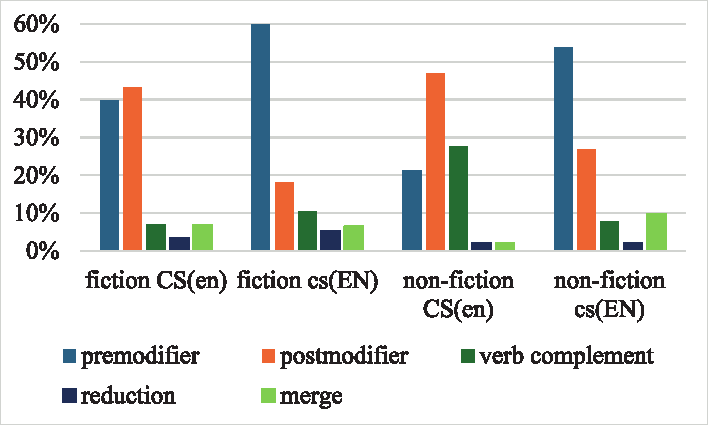
\includegraphics[width=\textwidth]{figures/4_Mala_figure 2mod.pdf}
\caption{\label{fig:mala:2}: The ratio (percentage) of classes of formally divergent correspondences across the registers and directions of translation.}
\end{figure}

The following section gives a more detailed description of the English non-prepositional counterparts of Czech postmodifying prepositional phrases. A larger corpus and a set of more specific queries (cf. 2.2) drawing on the above findings (3.2) were used to search for further instances of the types of correspondences outlined above.

\section{Non-prepositional English correspondences of Czech postmodifying prepositional phrases (Step 2)}
\subsection{Premodification}

Czech postmodifying PPs were found to correspond to several formal subtypes of English premodifiers:

\subsubsection{Premodification by a noun in English}

The English noun was the most frequent realization form of the premodifier corresponding to the Czech postmodifying PP. The premodifying function of the noun is signalled by its position; the partial conversion of the noun into a syntactic adjective is often accompanied by the loss of the contrast of number (\citealt{DuškováEtAl2009}: 2.22.21), e.g., cs. nejbohatší obchodníci \textit{s kořením, ořechy, zrny a lístky v Kóčínu} ‘the wealthiest merchants with spices, nuts, beans and leaves in Cochin’\textit{–} EN. the wealthiest \textit{spice, nut, bean and leaf} merchants in Cochin.

\newpage
This type of correspondence highlights some reasons why the prepositional form of postmodification may have been preferred to the more common adjectival premodification in Czech:

\begin{itemize}
\item  The adjectival premodifier may be blocked due to polysemy. For instance, what prevents the use of the adjective \textit{deskový} corresponding to \textit{record} in cs. obchod \textit{s deskami} ‘store with records’ \textit{–} EN. \textit{a record} store is the polysemy of the noun \textit{deska} in Czech. The adjective \textit{deskový} is derived from the noun when referring to a board or plate, e.g., \textit{desková} hra (‘board game’), \textit{desková} malba (‘panel painting’), \textit{desková} tektonika (‘plate tectonics’), but not when denoting a gramophone record.
\item  Another hindrance on using a premodifying adjective in Czech seems to be collocation. While the adjective \textit{datlový} (‘date’) collocates with several products made of dates, e.g., \textit{datlové} víno (‘date wine’), \textit{datlový} koláček (‘date cookie’), \textit{datlová} šťáva (‘date juice’) and occurs also in \textit{datlová} palma (‘date palm’), it does not seem to be used with date flour, e.g., CS. moučka \textit{z datlí} rozmíchaná v pivu – en. \textit{date} flour dissolved in beer.
\item  Another reason why a Czech postmodifying PP may be preferred to adjectival premodification consists in a possible shift in reference. While \textit{předsíňové} zrcadlo (‘the front-hall-\textsc{adj} mirror-\textsc{noun}’’) generally refers to a type of mirror,\footnote{Cf. the following example from the ‘House and Living’ magazine: \textit{V předsíňovém zrcadle se potřebujeme vidět od hlavy k patě}. ‘We need to see ourselves from head to toe in the front hall mirror’. (Dům a bydlení, 38/2017, Křen, Michal et al., 2022. \textit{Corpus SYN}, v. 11 from 14. 12. 2022. Institute of the Czech National Corpus, Charles University, Prague. Available from: https://www.korpus.cz)} zrcadlo \textit{v předsíni} (‘the mirror in the front hall’) has a specific reference, describing a particular item of furniture.
\item  The Czech postmodifying PP often corresponds to the English premodification by a proper noun, usually a place name, e.g., cs. v zapadlém a přísně tajném komplexu \textit{ve Virginii} ‘in the remote and classified complex in Virginia’\textit{–} EN. in the remote, classified \textit{Virginia} medical complex, and by compound nouns, often string compounds, e.g., CS. vídeňský spisovatel \textit{z přelomu století} ‘the Viennese writer from the turn of the century’ \textit{–} en. \textit{the turn-of-the-century} Viennese writer, cs. zprávy \textit{z bojišť} ‘news from the battlefields’\textit{–} EN. \textit{down-in-the-trenches} war stories.
\end{itemize}

A variety of semantic relations may obtain between the head noun and the Czech postmodifying PP corresponding to the English converted noun (the classification is based on \citealt{Hasselgård2021}: 150–151, cf. also \citealt{Malá2017}: 210–211), for instance:

\begin{itemize}
\item  temporal: cs. pohřebišti \textit{ze starší doby železné} ‘a burial from Late Iron Age’ \textit{–} EN. a \textit{Late Iron Age} burial, cs. nějakého strašidelného obchodního centra \textit{z přelomu století} ‘some creepy shopping mall from the turn of the century’ \textit{–} EN. some creepy \textit{turn-of-the-century} shopping mall;
\item  locative: CS. na zvlhlém koberci \textit{v obývacím pokoji} ‘on the wet carpet in the living room’ \textit{–} en. on their wet \textit{living-room carpet}, CS. slečny \textit{v baru} ‘girls in the bar’ \textit{–} en. the \textit{bar} girls, CS. jedné posluchárny \textit{v druhém patře} ‘one lecture room on the third floor’ \textit{–} en. one~of~the\textit{~third-floor~}lecture~rooms;
\item  focus: the modifier “specifies some aspect” of the head noun, for instance,
\begin{itemize}
\item the purpose, e.g., cs. pohádka \textit{na dobrou noc} ‘story for good night’ \textit{–} EN. \textit{bed-time} stories, CS. příspěvků \textit{v nezaměstnanosti} ‘benefits in unemployment’ \textit{–} en. \textit{unemployment} benefits, CS. nožíku \textit{na~rozřezávání~korespondence} ‘a knife for opening letters’ \textit{–} en. \textit{a letter} opener, cs. všechny její seznamy \textit{na nákup a vyřízení potřebných věcí} ‘all her lists for shopping and doing necessary things’ \textit{–} EN. all her \textit{shopping} lists and \textit{things-to-do} lists, cs. soutěž \textit{o nejlepší pojmenování letadla} ‘the competition for the best name for a plane’ \textit{–} EN. \textit{the best-name-for-a-plane} competition;
\item  content or composition, e.g., CS. kelímek \textit{s kafem} ‘the cup with coffee’ \textit{–} en. his \textit{coffee} cup, CS. krvavé paštiky \textit{z koňských jater} ‘blood-streaked pâté form horse liver’ \textit{–} en. blood-streaked \textit{horse liver} pâté, cs. salát \textit{z řas a chaluh} ‘the salad from seaweed’ \textit{–} EN. the \textit{seaweed} salad;
\item  occupation, e.g., CS. inteligentního obchodníka \textit{s chmelem} ‘the intelligent trader in hops’ \textit{–} en. the intelligent \textit{hops} trader, CS. továrník \textit{na umělé zuby} ‘the manufacturer for false teeth’ \textit{–} en. the \textit{false-teeth} manufacturer;
\end{itemize}
\item  attribute: the modifier “specifies a property of the NP head”, for instance,
\begin{itemize}
\item  material, e.g., CS. tajemné tramvaji \textit{ze zeleného mramoru} ‘the mysterious streetcar from green marble’ \textit{–} en. the mysterious \textit{green marble} streetcar, CS. dveře jídelny \textit{z mléčného skla} ‘the door of the dining-room from frosted glass’ \textit{–} en. \textit{frosted-glass} doors into the dining-room;
\item  cause, e.g., cs. nová alergie \textit{na sójové boby} ‘the new allergy to soya beans’ \textit{–} EN. the new \textit{soya-bean} allergy;
\item  size, e.g. cs. Východního sálu \textit{o rozloze téměř sto metrů čtverečních} ‘the East Room of the size almost one hundred square meters’\textit{–} EN. the \textit{thirty-two-hundred-square-foot} East Room.
\end{itemize}
\end{itemize}

\subsubsection{Premodification / determination by a genitive}

The correspondence between Czech postmodifying PPs and English nouns in the genitive case may illustrate another difference between the structure of noun phrases in both languages. The genitive serves either as a modifier or a determiner in the English noun phrase, and expresses a relatively broad range of semantic relations to the head noun. These relations are indicated by the prepositions in Czech (albeit loosely due to the polysemy of the prepositions), e.g., the locative determinative genitive corresponding to \textit{ve}{}-postmodification in Czech, cs. hospodářská činnost \textit{ve městě} ‘economic activity in the city’ \textit{–} EN. the \textit{city’s} economic activity, and a temporal modifying genitive, cs. úrok \textit{na tři měsíce} ‘interest for three months’ \textit{–} EN. \textit{three month’s} interest.

\subsubsection{Premodification by a denominal -\textit{ed} adjective}

The translation pair CS. plášť \textit{s kapucí} ‘raincoat with hood’ \textit{–} en. \textit{hooded} raincoat is similar to the English premodification by a converted noun. Here, however, the modifying function is indicated, apart from the position, by the denominal adjectival suffix -\textit{ed}. The adjectives are often derived from compound nouns, e.g., CS. jakýsi podivný anděl \textit{s psí hlavou} ‘a curious angel with a dog head’ \textit{–} en. a curious \textit{dog-headed} angel.

With animate head nouns, this type of modification typically describes the referent’s clothes or body-parts, e.g., cs. Bragg \textit{se svým bílým knírem} ‘Bragg with his white moustache’ \textit{–} EN. the \textit{white mustached} figure of Bragg, CS. žena \textit{s tlustými lýtky} ‘a woman with thick calves’ \textit{–} en. a \textit{heavy-thighed} [sic] woman, cs. pány \textit{v buřinkách} ‘men in bowler hats’ \textit{–} EN. the \textit{bowler-hatted} gentlemen, cs. lidé \textit{v maskách} ‘people in masks’ \textit{–} EN. the \textit{masked} individuals,  CS. barmana \textit{v bílém saku} ‘a barman in a white jacket’ \textit{–} en. a \textit{white-jacketed} barman. The referents of inanimate nouns are characterized by their shape or material, e.g., CS. vázy \textit{ve tvaru velblouda} ‘vases in the shape of a camel’ \textit{–} en. \textit{camel-shaped} vases, CS. nožem \textit{se zvláště širokým ostřím} ‘a knife with an especially broad blade’ \textit{–} en. a special \textit{broad-bladed} knife, cs. klobouk \textit{s pérem} ‘a hat with a feather’ \textit{–} EN. his \textit{feathered} hat, cs. psí bouda \textit{s plochou střechou} ‘a dog kennel with a flat roof’ \textit{–} EN. a \textit{flat-roofed} dog kennel, CS. židle \textit{s nízkými opěradly} ‘chairs with low backs’ \textit{–} en. \textit{low-backed} chairs. As the examples illustrate, the most frequent prepositions in this type of correspondence are \textit{s/se} ‘with’ and \textit{v/ve} ‘in’.

\subsubsection{Premodification by a past participle}

Examples like CS. první pytel \textit{s pískem} ‘the first bag with sand’ \textit{–} en. the first \textit{sand-filled} bag illustrate premodification by a compound which consists of a past participle and a noun representing the object or adverbial modifier of the verb (cf. bags \textit{filled with sand}).  The formation of a similar Czech type of compounds – deverbal adjectives – is more limited, and the transposition of the verbal action into a quality is expressed formally by an adjectival suffix \citep[133ff.]{bozdechova_tvoreni_1994}. The postmodifying PP appears to be a more flexible solution in Czech.

The participles often express a rather general relational meaning, corresponding to that indicated by the preposition, e.g., CS. pahýlem \textit{ve fusekli} ‘his arm in a sock’ \textit{–} en. his \textit{stocking-covered} arm, cs. koženým opaskem \textit{s náboji} ‘the leather belt with bullets’ \textit{–} EN. the \textit{bullet-laden} holster belt, cs. průmyslu \textit{na páru} ‘industry at steam’ \textit{–} EN. \textit{steam-driven} industry. Compounds with more specific meanings correspond to complex noun phrases complementing the Czech preposition, e.g., cs. prsty \textit{s okousanými nehty} ‘fingers with bitten nails’ \textit{–} EN. \textit{nail-bitten} fingers, CS. dálnic \textit{se zlatou vozovkou} ‘freeways with golden paving’ \textit{–} en. \textit{gold-paved} freeways.

\subsubsection{Other adjectival premodifiers}

Apart from the above recurrent counterparts, the Czech postmodifying PPs were also found to correspond to adjectival premodifiers. In translation pairs like CS. měsíc \textit{v úplňku} ‘moon in full’ \textit{–} en. \textit{full} moon, the modulation appears to be due to the absence of a corresponding Czech adjective and the fixed character of the naming unit in both languages (cf. also cs. život \textit{ve volné přírodě} ‘life in wild nature’\textit{–} EN. \textit{wild} life). Other instances seem to have been rather context-dependent choices, cf. the different translations of cs. tuhle příšernou cestu \textit{do Mexika} ‘this horrible trip to Mexico’ \textit{–} EN. this horrible \textit{Mexican} trip, and CS. svý cestě \textit{do Evropy} ‘his trip to Europe’ \textit{–} en. his trip \textit{to Europe}.

\subsection{Postmodification}

Czech postmodifying PPs can correspond to non-prepositional forms of postmodification in English. In most cases, the English postmodifier was a clausal one. The majority of these clauses were participial, often with semantically weak posture and relational verbs, which function as linking elements, similar to but more explicit than the corresponding Czech prepositions, e.g., CS. sochy \textit{s lampama} ‘statues with lamps’ \textit{–} en. the statues \textit{bearing lamps}, CS. vory \textit{s bronzovými lvy} ‘rafts with bronze lions’ \textit{–} en. rafts \textit{carrying bronze lions}, CS. pecí \textit{z žáruvzdorných cihel} ‘ovens from fire-resistant bricks’ \textit{–} en. ovens \textit{built of fire-resistant brick}, cs. rovných červených kachlů \textit{ve staré římské konstrukci} ‘flat red tiles in the ancient Roman structure’ \textit{–} EN. flat red tiles \textit{placed in the ancient Roman structure}.

The same type of predicates was attested in finite postmodifying clauses, e.g., CS. ukazováčkem \textit{s prstenem ze starého zlata} ‘an index finger with a ring from antique gold’ \textit{–} en. an index finger \textit{that wore an antique gold ring}, CS. obrovský rudý transparent \textit{s nápisem} […] ‘a huge red banner with an inscription’ \textit{–} en. a huge red banner \textit{that read} […].

Another type of non-finite postmodifying clause was infinitival clauses, which usually complement a de-verbal noun, e.g., CS. snahy \textit{o formalizaci teorie} ‘attempts at the formalization of theory’ \textit{–} en. attempts \textit{to formalise theory}.

Other forms of postmodifiers – adverbs, adjectives and appositive nouns – were represented marginally, e.g., cs. trávy \textit{na druhém břehu} ‘the grass on the opposite bank’ \textit{–} EN. the grass \textit{beyond}, cs. zálivu Guantánamo \textit{na Kubě} ‘bay Guantánamo in Cuba’ \textit{–} EN. \textit{Guantánamo Bay, Cuba}.

\subsection{Verb complements}

Example \REF{ex:mala:8} illustrates the Czech noun phrase with a deverbal head-noun \textit{porady} (‘consultation’) complemented by a PP \textit{s Hlavounem}. The English counterpart relies on a non-finite verb form, the gerund \textit{consulting}, complemented by the object \textit{Bigwig}. The form of the complement is based on the valency of the de-verbal noun and the verb, respectively.

\ea\label{ex:mala:8}
cs. Rozhodl se zamířit do lesa bez \textit{porady s Hlavounem} [without a consultation with Bigwig][…] (transl. by Jitka Minaříková)\\
EN. He decided to go straight into the wood without \textit{consulting Bigwig} […] (Richard Adams, Watership down, fiction)
\z

Czech de-verbal nouns with prepositional complements typically correspond to non-finite or finite clauses. The non-finite counterparts can be exemplified by further gerund constructions, e.g., CS. \textit{zapomenutí na vláčné pohyby ruky} ‘forgetting-\textsc{noun} about the supple movements of the hand’ \textit{–} en. \textit{forgetting the supple movements of the hand}, CS. \textit{sňatku s lenochem} ‘marriage with a loafer’ \textit{–} en. \textit{marrying a loafer}, participial clauses, e.g., CS. \textit{satiry na jejich ideologii, puritanismus} ‘satire of their ideology, puritanism’ \textit{–} en. \textit{satirising their puritan ideology}, or infinitive clauses, e.g., cs. \textit{učinit ústupek ze své osobní integrity} ‘make a compromise from his personal integrity’ \textit{–} EN. \textit{to compromise his personal integrity}, cs. \textit{výpravu do zahrady} ‘a raid on a garden’\textit{–} EN. \textit{to raid a garden}. The correspondences CS. \textit{se zřetelem k frekvenci} ‘with consideration to frequency’ \textit{–} en. \textit{considering the frequency}, and CS. \textit{v návaznosti na K. Buhlera} ‘in connection with K. Buhler’ \textit{–} en. \textit{following K. Buhler} may illustrate the recategorization of the ‘preposition + noun + preposition’ construction into a secondary preposition in Czech, mirrored by a de-participial preposition in English.

Translation with a finite clause requires a greater extent of restructuring \REF{ex:mala:9}, which also involves filling the position of the subject in English. The \textit{s-}PP can correspond to the verb \textit{have} expressing a general meaning of belonging. Example \REF{ex:mala:10} illustrates the use of the semantically weak verb \textit{have} with an inanimate locative subject \citep{mala_english_2019}.

\ea\label{ex:mala:9}
CS. Přímou vládu \textit{v Čechách a na Moravě} [‘direct rule in Bohemia and Moravia] císař nikdy nevykonával […] (Jaroslav Pánek et al., Dějiny českých zemí, non-fiction)\\
en. The Emperor never directly ruled \textit{Bohemia and Moravia} […] (transl. by Petra Key et al.)
\z

\ea\label{ex:mala:10}
CS. Po celé délce pokoje se táhl tmavý stůl, kolem něho stály v pravidelných rozestupech vysoké židle \textit{s černým koženým polstrováním} [‘tall chairs with black leather upholstery’], přitlučeným k dřevu mohutnými kovovými cvočky. (Michal Ajvaz, Prázdné ulice, fiction) \\
en. Running the whole length of the room was a dark table with tall chairs at regular intervals around it. These chairs \textit{had black-leather upholstery} attached to the seat with mighty metal studs. (transl. by Andrew Oakland)
\z

\subsection{Reduction and merger}

The English counterparts resulting from the last two types of correspondence – (syntactic) reduction and merger – look similar; each of them, however, is a result of a different process. Reduction consists in the English version lacking the counterpart of the Czech head noun, without a substantial difference in the meaning of the noun phrase, e.g., cs. vyrazily \textit{lidem v prvních řadách} dech ‘people in the front rows’ – EN. drew a gasp from \textit{the front row}, cs. nic tak radikálního jako \textit{život v Atlantě} ‘life in Atlanta’ – EN. nothing as radical as \textit{Atlanta}, cs. \textit{ryba na předloze} ‘the fish in the original’ – EN. \textit{the original}. The meaning of the head noun is generally derivable from the context; what is retained is the rhematic part of the noun phrase, carrying the most important, focal piece of information within the noun phrase.

The head noun and the prepositional postmodfier can be merged in two ways: the first, illustrated by the translation pairs cs. \textit{chuť k jídlu} ‘appetite for food’\textit{–} EN. \textit{appetite}, CS. \textit{do rýhy ve výstřihu} ‘down the line in her cleavage’ \textit{–} en. \textit{down her cleavage}, or cs. \textit{vyhození mince do vzduchu} ‘the flip of a coin in the air’ \textit{–} EN. \textit{the flip of a coin}, involves the same idea in both languages expressed in English using a different, often univerbal, expression. The second type most often resembles the PP corresponding to premodification by a noun (4.1.1). Here the nominal modifier becomes integrated with the head noun as the initial stem of a compound, e.g., cs. \textit{truhlík na uhlí} ‘the scuttle for coal’ \textit{–} EN. \textit{the coal-scuttle}, cs. \textit{hodiny s vestavěným rádiem} ‘a clock with inbuilt radio’ \textit{–} EN. \textit{a clock-radio}, cs. \textit{pastičky na myši} ‘traps for mice’\textit{–} EN. \textit{mousetraps}, cs. \textit{police s knihami} ‘shelves with books’ \textit{–} EN. \textit{bookshelves}. Alternatively, the English noun can be formed by derivation, adding a suffix that denotes a person, similarly to the Czech head noun, e.g., cs. \textit{obchodníci s látkami} ‘traders in cloth’ \textit{–} EN. \textit{clothiers}.

\section{Concluding remarks}

The Czech postmodification realized by a PP rarely has a divergent translation counterpart. Non-prepositional counterparts were attested in 23.4\% of (1,000) postmodifying PPs. The highest incidence of formally non-congruent correspondences was observed in Czech translations of English fiction; in non-fiction, generally, formally divergent counterparts were less frequent than in fiction. The majority of formally congruent counterparts (92.2 \%) also performed the same, postmodifying syntactic function as the Czech PPs. The extent of syntactic divergence was largest between English original fiction texts and their Czech translations (cs(EN)).

The degree of cross-linguistic correspondence and the preference for a particular type of counterpart seem to be influenced by the direction of translation here. The proportion of non-congruent counterparts was larger in the cs(EN) direction both in fiction and non-fiction texts. In this direction, the most prominent divergent EN sources of Czech postmodifying PPs were premodifiers realized by nouns, a construction which has no direct congruent counterpart in the Czech language, e.g., EN. \textit{cool stream water} translated as cs. \textit{voda z chladného pramene} ‘water from cool stream’. In the opposite, Czech > English direction (CS(en)), the translators appeared to rely more frequently on postmodifying clauses as the counterparts of Czech postmodifying PPs.

One of the goals of the present study was to try to shed some light on the motivation for the translation divergence. Most of the systematic differences seem to be ascribable to the predominantly analytic character of the English language, compared to predominantly synthetic Czech. English has available to it several means of expressing modification that have no formally congruent counterparts in Czech. These include the most frequent divergent counterpart of Czech postmodifying PPs – premodification by a noun. Recurrent ‘noun + noun’ combinations tend to form compounds. The process, which was classified here as merging the head noun and the modifier, can alternatively be viewed as a scale, with premodifying nouns at one end, and compounds at the other. The transposition between the English premodifying noun (phrase) and the Czech postmodifying PP is fairly straightforward. The relationship between the head of the noun phrase and the modifier is retained, no shift from one word-class to another is needed, nor does the syntactic transposition pose major restrictions on the complexity of the modifying noun phrase. The Czech preposition renders the relationship between the head and the modifier more explicit than the juxtaposition in English.

Another feature typical of English (in comparison with Czech) is the abundance of non-finite verb forms. Participles, gerunds and infinitives may act as counterparts of either the postmodifying PP or of the head of the noun phrase. The postmodifying function is typically performed by semantically weak verbs in the present or past participial form, which easily recategorize into secondary prepositions. In this respect, the participial postmodifiers resemble the Czech primary prepositions – both serve as elements that link the head noun to the noun phrase in postmodification, conveying quite broad meanings, such as composition, material, or accompanying circumstance. Czech, as a predominantly synthetic language, generally relies heavily on verb inflection. Participial verb forms are therefore rare. The construction structurally closest to English postmodifying participles is the Czech deverbal adjective, which has to agree with the head noun in gender, number and case, expressed by the adjectival suffix. The Czech postmodifying PP, requiring no formal concord with the head noun, therefore appears to be a more felicitous solution here as long as the simple primary preposition is capable of capturing the relationship between the nouns indicated by the English participle.

The use of the modifying or determinative genitive as the counterpart of the Czech postmodifying PP highlights the differences in the structure of the noun phrase between the two languages. At the same time, in the inflectionally poor English, the genitive is capable of expressing a relatively broad range of meanings, and it combines with both animate and inanimate nouns. In Czech, the corresponding semantic relations between the head noun and the modifier may be expressed more explicitly by the preposition.

The choice of a particular type of counterpart was shown to impact on how explicitly the semantic relationship between the head noun and the modifier is expressed. Premodification by a noun, with syntactic relations indicated merely by word-order, leaves the semantic relationship implicit in English. The modifying function of denominal adjectives and participial premodifiers is signalled, apart from the position, morphologically, but there is no explicit indicator of the semantic relation between the modifier and the head. In postmodifying clauses, it is often the semantically weak (non-finite) verb that serves as a more explicit equivalent of the Czech preposition, linking the head noun to another noun phrase and expressing the semantic relation between them. As shown in \sectref{sec:mala:3.2}, the universal trend towards increased explicitness in translation (cf., e.g., \citealt{BernardiniRusso2018}), seems to assert itself in both directions of translation. In the English > Czech direction, the Czech preposition marks the semantic relation between the head noun and the modifying noun phrase explicitly, compared to the most frequent English source construction, premodification by the noun juxtaposed to the head.  In the opposite, Czech > English direction, the translators were found to rely most often on English postmodifying clauses, whose predicates indicate the semantic relation between the head noun and the modifying noun phrase more explicitly than the corresponding Czech preposition.

The above observations may suggest some reasons for the divergent correspondences. They are, however, tendencies rather than rigorously observed rules. As examples \REF{ex:mala:11} and \REF{ex:mala:12} below illustrate, the choice between the prepositional and non-prepositional English counterparts of the Czech postmodifying PPs may be context-dependent, leaving the decision open for the translator.

\ea\label{ex:mala:11}
CS. Na druhé straně chodby stály ve výklencích sochy \textit{z bílého mramoru} [statues of white marble]; […] (Michal Ajvaz, Zlatý věk, fiction)\\
en. In alcoves on the other side of the corridor there are statues \textit{of white marble}; […] (transl. by Andrew Oakland)
\z

\ea\label{ex:mala:12}
CS. […] přesně na tom místě […] stál teď pomník \textit{z černého mramoru} [a headstone of black marble] s docela jiným pozlaceným jménem. (Milan Kundera, Směšné lásky, fiction)\\
en. […] precisely on that spot […] now stood \textit{a black marble} headstone with a quite different name in gilt. (transl. by Suzanne Rappaport)\\
\z

Even though the present chapter focussed on a minor type of translation correspondence between Czech and English, it is hoped to have catalogued the recurrent patterns and suggested some motivation for the choice of a particular counterpart. To give a comprehensive picture, however, the correspondences between English PPs and their Czech translations should also be explored in detail both in cs(EN) and CS(en). More research is needed to situate the results within the broader area of translation correspondences between Czech and English at the level of the noun phrase in fiction and non-fiction.

Drawing on parallel translation corpora, this chapter also highlights the importance of sufficient reliable bi-directional data to explore infrequent phenomena.

\sloppy\printbibliography[heading=subbibliography,notkeyword=this]
\end{document}
